\documentclass[
	classe=$2^{de}$,
	headerTitle=Cours\space Chapitre\space 7
]{coursclass}

\usepackage{tikz-repère}
\usepackage{tkz-tab}
\usetikzlibrary{automata,calc,positioning}

\title{Chapitre 7 : Fonctions}
\date{}
\author{}

\begin{document}

\maketitle

\begin{definition}[Fonction, image, antécédent]
	Une \textbf{fonction} est un procédé qui à un nombre réel $x$ associe un unique nombre réel $f(x)$.

	\begin{minipage}{0.65\textwidth}
		\begin{itemize}
			\item $f(x)$ est \textbf{L'image} de $x$ par la fonction $f$. On représente une image par la lettre $y$, et on écrit alors

			      $$ f(x) = y $$
			\item $x$ est \textbf{UN antécédent} de $y$.
		\end{itemize}
	\end{minipage}
	\begin{minipage}{0.3\textwidth}
		\hspace{2em}
		\begin{tikzpicture}
			\node (X) {$x$};
			\node (F) [right=of X] {};
			\node (Y) [right=of F] {$f(x)$};
			\path[\myArrow] (X) edge node[above] {$f$} (Y);
		\end{tikzpicture}
	\end{minipage}
\end{definition}

\begin{remarque}
	\begin{itemize}
		\item Il n'y a \uline{qu'une seule image} pour un nombre donné.
		\item Il peut y avoir \uline{plusieurs antécédents} pour un nombre donné.
	\end{itemize}
\end{remarque}

\begin{definition}[Calcul d'image]
	Si on a une expression \textbf{algébrique} de la fonction $f$, on peut calculer l'image d'un nombre en remplaçant $x$ par ce nombre dans l'expression de la fonction.
\end{definition}

\begin{exemple}
	Si $f$ est la fonction qui à $x$ associe $3x + 2$ :
	\begin{itemize}
		\item $f(2) = 3×2 + 2 = 8$
		\item Attention : si on remplace $x$ par une expression complexe, il faut ajouter des parenthèses. Par exemple,

		      $f(1 + 3) = 3×(1 + 3) + 2 = 3×4 + 2 = 14$
	\end{itemize}
\end{exemple}

\begin{definition}[Domaine de définition]
	L'ensemble des nombres ayant une image par la fonction $f$ est appelé le \textbf{domaine de définition} de $f$. On le note $𝒟_f$.
\end{definition}

\begin{exemple}
	\begin{itemize}
		\item Si $f$ est la fonction qui à $x$ associe $\dfrac{1}{x}$, alors $x$ ne peut pas être $0$.

		      Son domaine de définition est $𝒟_f = \intervalle{]}{-∞}{0}{[} ∪ \intervalle{]}{0}{+∞}{[}$.
		\item Si $f$ représente une longueur, $x$ ne peut pas être négatif.

		      Son domaine de définition est $𝒟_f = \intervalle{[}{0}{+∞}{[}$.
	\end{itemize}
\end{exemple}

\newpage

\begin{definition}[Courbe représentative]
	La \textbf{courbe représentative} d'une fonction $f$ est l'ensemble des points $(x ; y)$ tels que $y = f(x)$.
\end{definition}

\begin{definition}[fonction affine]
	Une \textbf{fonction affine} est une fonction définie par
	$$ f(x) = mx + p $$
	où $m$ et $p$ sont des nombres réels fixés.
\end{definition}

\begin{remarque}
	\begin{itemize}
		\item Si $p = 0$, on a alors $f(x) = mx$, donc la fonction est \textbf{linéaire}.
		\item Si $m = 0$, on a alors $f(x) = p$, donc la fonction est \textbf{constante}.
	\end{itemize}
\end{remarque}

\begin{definition}[Coefficient directeur et ordonnée à l'origine]
	Soit $f(x) = mx + p$ une fonction affine. Alors
	\begin{itemize}
		\item $m$ est le \textbf{coefficient directeur} (ou la \textbf{pente}) de la droite représentative de $f$.
		\item $p$ est l'\textbf{ordonnée à l'origine}.
	\end{itemize}
\end{definition}

\begin{exemple}
	\begin{minipage}{0.4\textwidth}
		\begin{center}
			\begin{tikzpicture}[scale=0.7]
				\tikzRepere{-0.5}{4.5}{-0.5}{9.5}
				\draw[domain=-1:5,very thick,blue] plot({\x},{1.5*\x + 2});
				\draw[very thick,mygreen] (0,2) -- ++(-0.2,0) node[left] {$p$};
				\draw[thick,red] (2,5) -- node[midway,below] {$1$} ++(1,0) -- node[midway,right] {$m$} ++(0,1.5);
			\end{tikzpicture}
		\end{center}
	\end{minipage}\hspace{0.05\textwidth}
	\begin{minipage}{0.5\textwidth}
		La droite ci-contre correspond à la fonction
		\begin{align*}
			f(x) & = mx + p   \\
			     & = 1,5x + 2
		\end{align*}
	\end{minipage}
\end{exemple}

\begin{propriete}[Représentation d'une fonction affine]
	La représentation graphique d'une fonction affine est une droite.
\end{propriete}

\begin{definition}[Variations d'une fonction]
	On considère une fonction $f$ définie sur un intervalle $I$.
	\begin{itemize}
		\item On dit que $f$ est \textbf{croissante} sur $I$ si pour tout réels $a$ et $b$ de $I$ tels que $a ≤ b$, on a $f(a) ≤ f(b)$.
		\item On dit que $f$ est \textbf{décroissante} sur $I$ si pour tout réels $a$ et $b$ de $I$ tels que $a ≤ b$, on a $f(a) ≥ f(b)$.
	\end{itemize}
\end{definition}

\begin{exemple}
	\directlua{
		function draw_path(f, a, b)
		tex.print("\\draw[thick,red,dashed] (", a, ",0) node[below] {$a$} -- (", a, ",", f(a), ") -- (0,", f(a), ") node[left] {$f(a)$};")
		tex.print("\\draw[thick,red,dashed] (", b, ",0) node[below] {$b$} -- (", b, ",", f(b), ") -- (0,", f(b), ") node[left] {$f(b)$};")
		end
	}
	\begin{minipage}{0.45\textwidth}
		\begin{center}
			\begin{tikzpicture}[scale=0.7]
				\tikzRepere{-1}{3}{-1}{3}[][]
				\draw[thick,blue,domain=-1:3] plot({\x},{exp(\x - 2)});
				\directlua{draw_path(function (x) return math.exp(x - 2) end, 1.5, 2.5)}
			\end{tikzpicture}

			On a $a ≤ b$, et $f(a) ≤ f(b)$,

			donc $f$ est croissante.
		\end{center}
	\end{minipage}\hspace{0.05\textwidth}
	\begin{minipage}{0.45\textwidth}
		\begin{center}
			\begin{tikzpicture}[scale=0.7]
				\tikzRepere{-1}{3}{-1}{3}[][]
				\draw[thick,blue,domain=-1:3] plot({\x},{-exp(\x - 2) + 2});
				\directlua{draw_path(function (x) return -math.exp(x-2)+2 end, 1, 2.2)}
			\end{tikzpicture}

			On a $a ≤ b$, et $f(a) ≥ f(b)$,

			donc $f$ est décroissante.
		\end{center}
	\end{minipage}
\end{exemple}

\begin{greybox}[frametitle={Tableau de variations}]
	Un \textbf{tableau de variations} résume les intervalles sur lesquelles la fonction est croissante ou décroissante :

	\begin{minipage}{0.45\textwidth}
		\begin{center}
			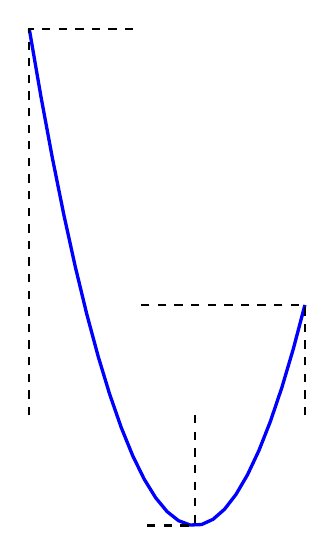
\begin{tikzpicture}[scale=0.7]
				\tikzRepere{-3}{3}{-2}{7}
				\draw[very thick,blue,domain=-2:3] plot({\x},{\x*\x - 2*\x - 1});
				\foreach \x/\y in {-2/7,1/-2,3/2} {
						\draw[thick,dashed] (\x,0) -- ++(0,\y) -- (0,\y);
					}
			\end{tikzpicture}
		\end{center}
	\end{minipage}\hspace{0.05\textwidth}
	\begin{minipage}{0.45\textwidth}
		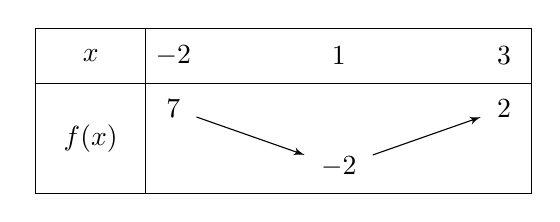
\begin{tikzpicture}[scale=0.7]
			\tkzTabInit{$x$ / 1 , $f(x)$ / 2}{$-2$, $1$, $3$}
			\tkzTabVar{+/ $7$, -/ $-2$, +/ $2$}
		\end{tikzpicture}
	\end{minipage}
\end{greybox}

\end{document}
